\documentclass[10pt,twocolumn]{article}
\usepackage{candor}
\begin{document}

\title{{\bf Fantastic Adventures Involving \rpoS, Baby}}
\author{{\sc H. Lian, V. Bhattcharya, and D.R. Vitek}}
\date{{\sc \today}}
\maketitle

\section{Analyzing \rpoS}

We know {\it Escherichia coli} translationally regulates~\cite{rpos:process} RNA polymerase sigma factor \rpoS,
whence we may analyze potential areas of the sequence where transcriptional regulation can occur and
suggests sequence changes to improve protein yield.

\subsection{Polar Plot}

The polar plot for \rpoS\ (Figure~\ref{rpos:polar}) is similar to those for other normal genes; 
it remains near the species angle.

\begin{figure}[htp]
    \centering
    \caption{Original \rpoS\ Sequence}
    \label{rpos:polar}
    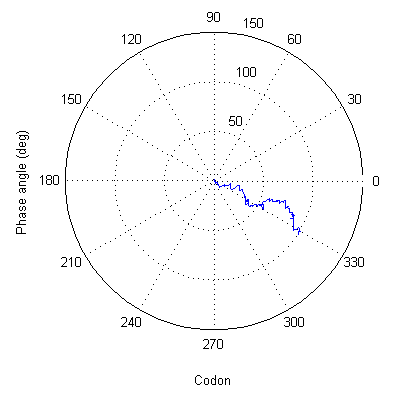
\includegraphics[scale=0.7]{rpoS/polar.png}
\end{figure}

\subsection{Displacement Plots}

Unexpectedly, the displacement plot for \rpoS\ (Figure~\ref{rpos:disp}) does not show any interesting behavior.
The displacement stays within the range $[-0.5,0.5]$, which is well outside the trouble region of $\pm 1$.

\begin{figure}[htp]
    \centering
    \caption{Original \rpoS\ Displacement Plot}
    \label{rpos:disp}
    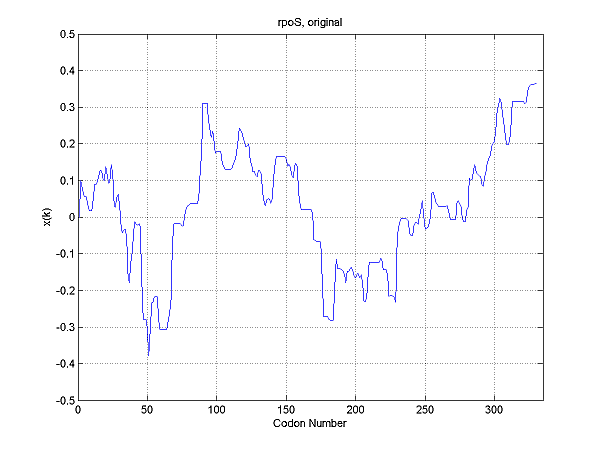
\includegraphics[scale=0.7]{rpoS/original.png}
\end{figure}

On a more sensitive but still stochastic model, however, \rpoS\ shows a different displacement plot.  
Figure~\ref{rpos:sensdisp} shows a graph of ten iterations. It indicates two areas where frameshifts may occur,
the first approximately at codon 95, when the displacement plot nears one, which one iteration demonstrates
its exceeding 1.5 in displacement. The other lies approximately at codon 180; where the displacement dips near negative one.

\begin{figure}[htp]
    \centering
    \caption{Original \rpoS\ on a Sensitive Model}
    \label{rpos:sensdisp}
    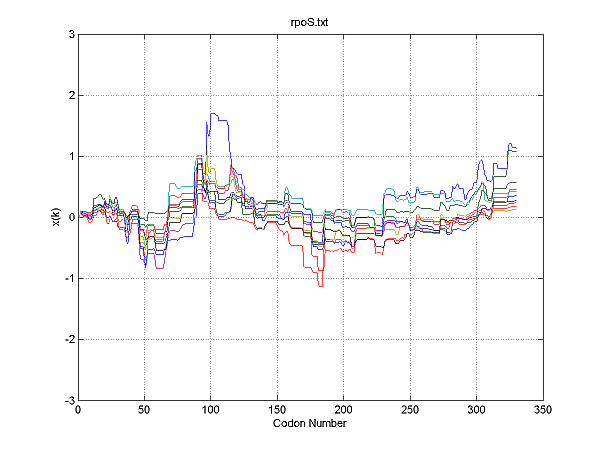
\includegraphics[scale=0.7]{rpoS/sensitive.png}
\end{figure}

\section{Without Frameshifts}

With a brute-force algorithm, substituting 33 synonymous codons in the \rpoS\ sequence minimizes
the deviation of \rpoS\ displacement toward $\pm 1$ on the sensitive model, potentially reducing
possible mistake frameshifts during translation.

\subsection{Displacement and Polar Plots}

On the less sensitive model, a displacement plot for the improved sequence (Figure~\ref{rposmax:disp})
indicates less variation compared to Figure~\ref{rpos:disp}. The more sensitive model accentuates this
difference (Figure~\ref{rposmax:sensdisp} versus Figure~\ref{rpos:sensdisp}).

\begin{figure}[htp]
    \centering
    \caption{Modified \rpoS Displacement Plot}
    \label{rposmax:disp}
    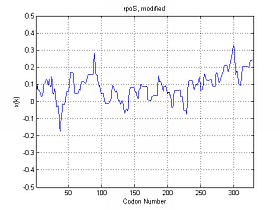
\includegraphics[scale=1]{rpoS/max.png}
\end{figure}

\begin{figure}[htp]
    \centering
    \caption{Modified \rpoS\ on a Sensitive Model}
    \label{rposmax:sensdisp}
    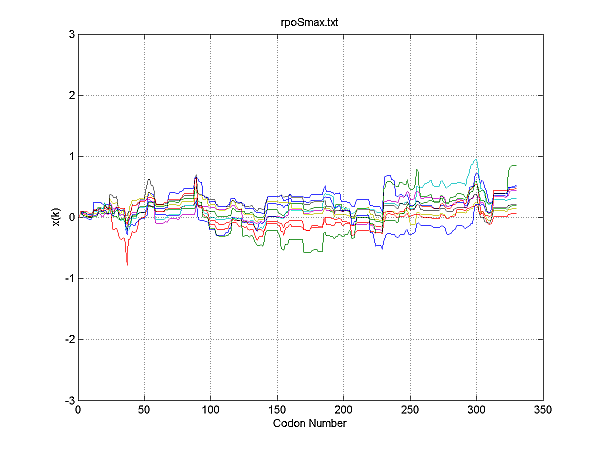
\includegraphics[scale=0.7]{rpoS/max-sensitive.png}
\end{figure}

The polar plot (Figure~\ref{rposmax:polar}) stays closer to the species angle as well,  
avoiding the large deviation starting about halfway down the sequence shown in the original polar plot (Figure~\ref{rpos:polar}).

\begin{figure}[htp]
    \centering
    \caption{Modified \rpoS\ Polar Plot}
    \label{rposmax:polar}
    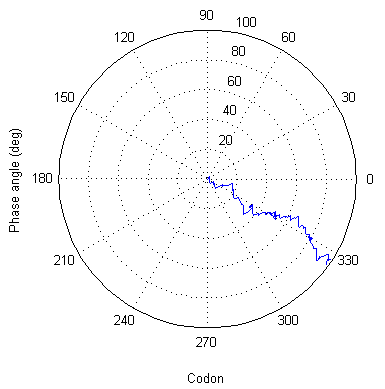
\includegraphics[scale=0.7]{rpoS/max-polar.png}
\end{figure}

\subsection{Yields}

After 5000 iterations on the sensitive model, the original \rpoS\ sequence
ran from start to finish without frameshift mistakes 39.8\% of the time compared to
88.6\% for the improved sequence. The models also reported an average standard deviation from zero of
0.3831 compared to the 0.2235 for the modified sequence, the lower deviation again
indicating a smaller likelihood of a mistake frameshift.

\section{A Frameshifting Sequence}

The previous section proposed a sequence to reduce deviation from the zero axis by changing 33 codons.
This section proposes a programmed frameshift with only 3 codon changes, tendering similar results.

\subsection{Plots}

On the less sensitive model, both plots contain similarities to plots of the known frameshifter \prfB,
including the polar plot (Figure~\ref{rposfs:polar}).
The dips in the displacement plot occur approximately at codons 50 and 180 (Figure~\ref{rposfs:disp});
the latter trouble spot corresponds, nota bene, to the original sequence.
The trouble spot at codon 90 remains as a bulge above the horizontal line $x(k)=2$,
but less prominently.

% What does properly entail?
On a sample of 1000 iterations, the proper frameshift occurs 86\% of the time,
but the sequence runs properly only 55.1\% of the time.

\begin{figure}[htp]
    \centering
    \caption{Frameshifting \rpoS\ Displacement Plot}
    \label{rposfs:disp}
    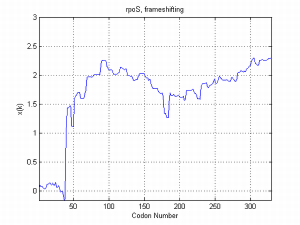
\includegraphics{rpoS/frameshift.png}
\end{figure}

\begin{figure}[htp]
    \centering
    \caption{Frameshifting \rpoS\ Polar Plot}
    \label{rposfs:polar}
    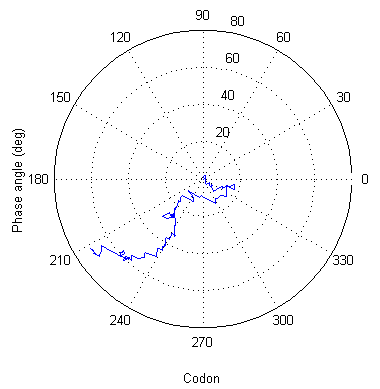
\includegraphics[scale=0.7]{rpoS/frameshift-polar.png}
\end{figure}

\bibliography{wizards}
\end{document}